
                        \documentclass{article}
                        \usepackage{tikz}
                        \usetikzlibrary{automata, positioning}

                        \begin{document}
                        \section{}

                            \begin{center}
                                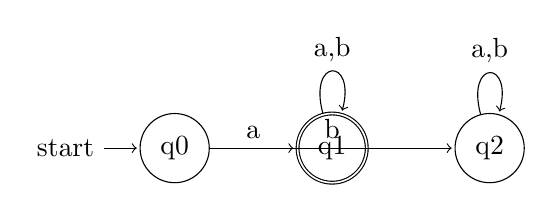
\begin{tikzpicture}[shorten >=1pt, node distance=2cm, on grid, auto] 
                    
    \node [state,initial] (q0) at (0 , 0) { q0};
    \node [state,accepting] (q1) at (2 , 0) { q1};
    \node [state] (q2) at (4 , 0) { q2};
 \path[->]
      (q0) edge node {a} (q1)
      (q0) edge node {b} (q2)
      (q1) edge[loop above] node {a,b} (q1)
      (q2) edge[loop above] node {a,b} (q2);
                        \end{tikzpicture}
                        \end{center}
                        \end{document}
                        